\documentclass[%
preprint,
 amsmath,
 amssymb,
 aps,
]{revtex4-2}

\usepackage{graphicx}% Include figure files
\usepackage{dcolumn}% Align table columns on decimal point
\usepackage{bm}% bold math
\usepackage{lipsum}
\usepackage{physics}


\bibliographystyle{apsrev4-2}

\begin{document}

\preprint{APS/123-QED}
\title{Manuscript Title:\\Sub-Title of manuscript }% Force line breaks with \\

\author{author1}%
 \affiliation{Authors' institution and/or address}%
 \email{email@address.tbd}
\author{author1}%
\affiliation{%
Authors' institution and/or address}%


\date{\today}

\begin{abstract}
\lipsum[1]
\end{abstract}

\maketitle


\section{Section 1}

\lipsum[1-4] Fake citation.

\subsection{Subsection 1}

\lipsum[1-4]

Workflow-ul modelului.

\begin{figure*}[h]
    \centering
    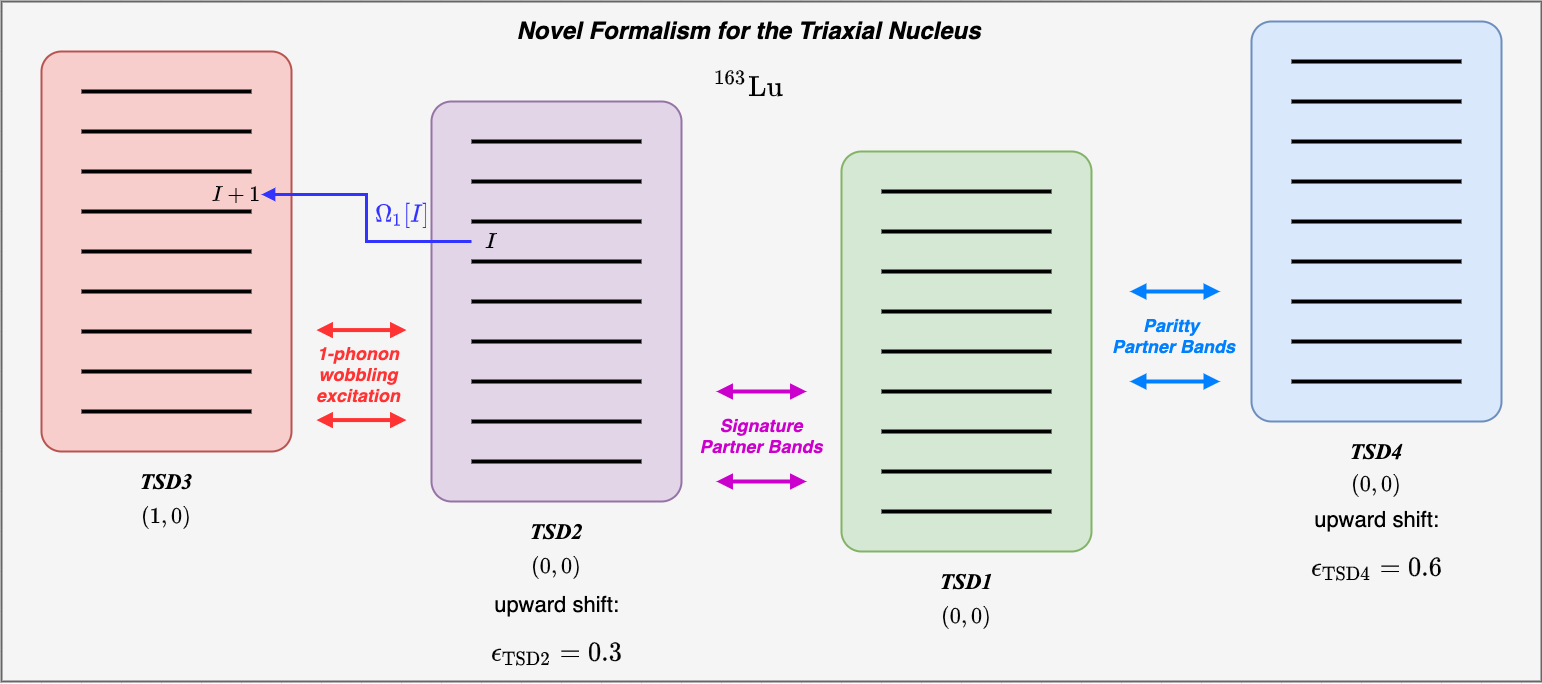
\includegraphics[width=0.95\textwidth]{./images/diagrams/double_shift_fit_workflow.png}
    \caption{New approach}
    \label{fig:band-structure}
\end{figure*}



\bibliography{biblio}% Produces the bibliography via BibTeX.

\end{document}
